\documentclass[t]{beamer}
\usepackage{beamerthemesplit}
\usepackage{xcolor}
\usepackage{color}
\usepackage{colortbl}
\usetheme{USC}
\begin{document}

\graphicspath{ {../Manuscript/figures/}{Graphics/} }

\title[USC Viterbi School of Engineering]{Probabilistic estimation of link travel times in dynamic road networks}  
\author[Mohammad Asghari]{Mohammad Asghari\\ \small{masghari@usc.edu}\\ \vspace{0.1in} \tiny{Joint work with Tobias Emrich, Ugur Demiryurek and Cyrus Shahabi}}

\date{Nov 6, 2015} 

\begin{frame}
\titlepage
\begin{columns}
  \column{.2\textwidth}
  \begin{center}
    
\includegraphics[height=1.5cm]{viterbi_logo.jpg}
  \end{center}
  \column{.6\textwidth}
  \column{.2\textwidth}
  \begin{center}
    
\includegraphics[height=1.5cm]{imsc_logo.jpg}   
  \end{center}
\end{columns} 
\end{frame}

\begin{frame}\frametitle{Outline}\tableofcontents
\end{frame} 

\section{Introduction}
\begin{frame}\frametitle{Motivation}
\vspace{-0.2in}
\only<1-2>{
\begin{columns}
	\column{0.5\textwidth}
		\begin{center}
			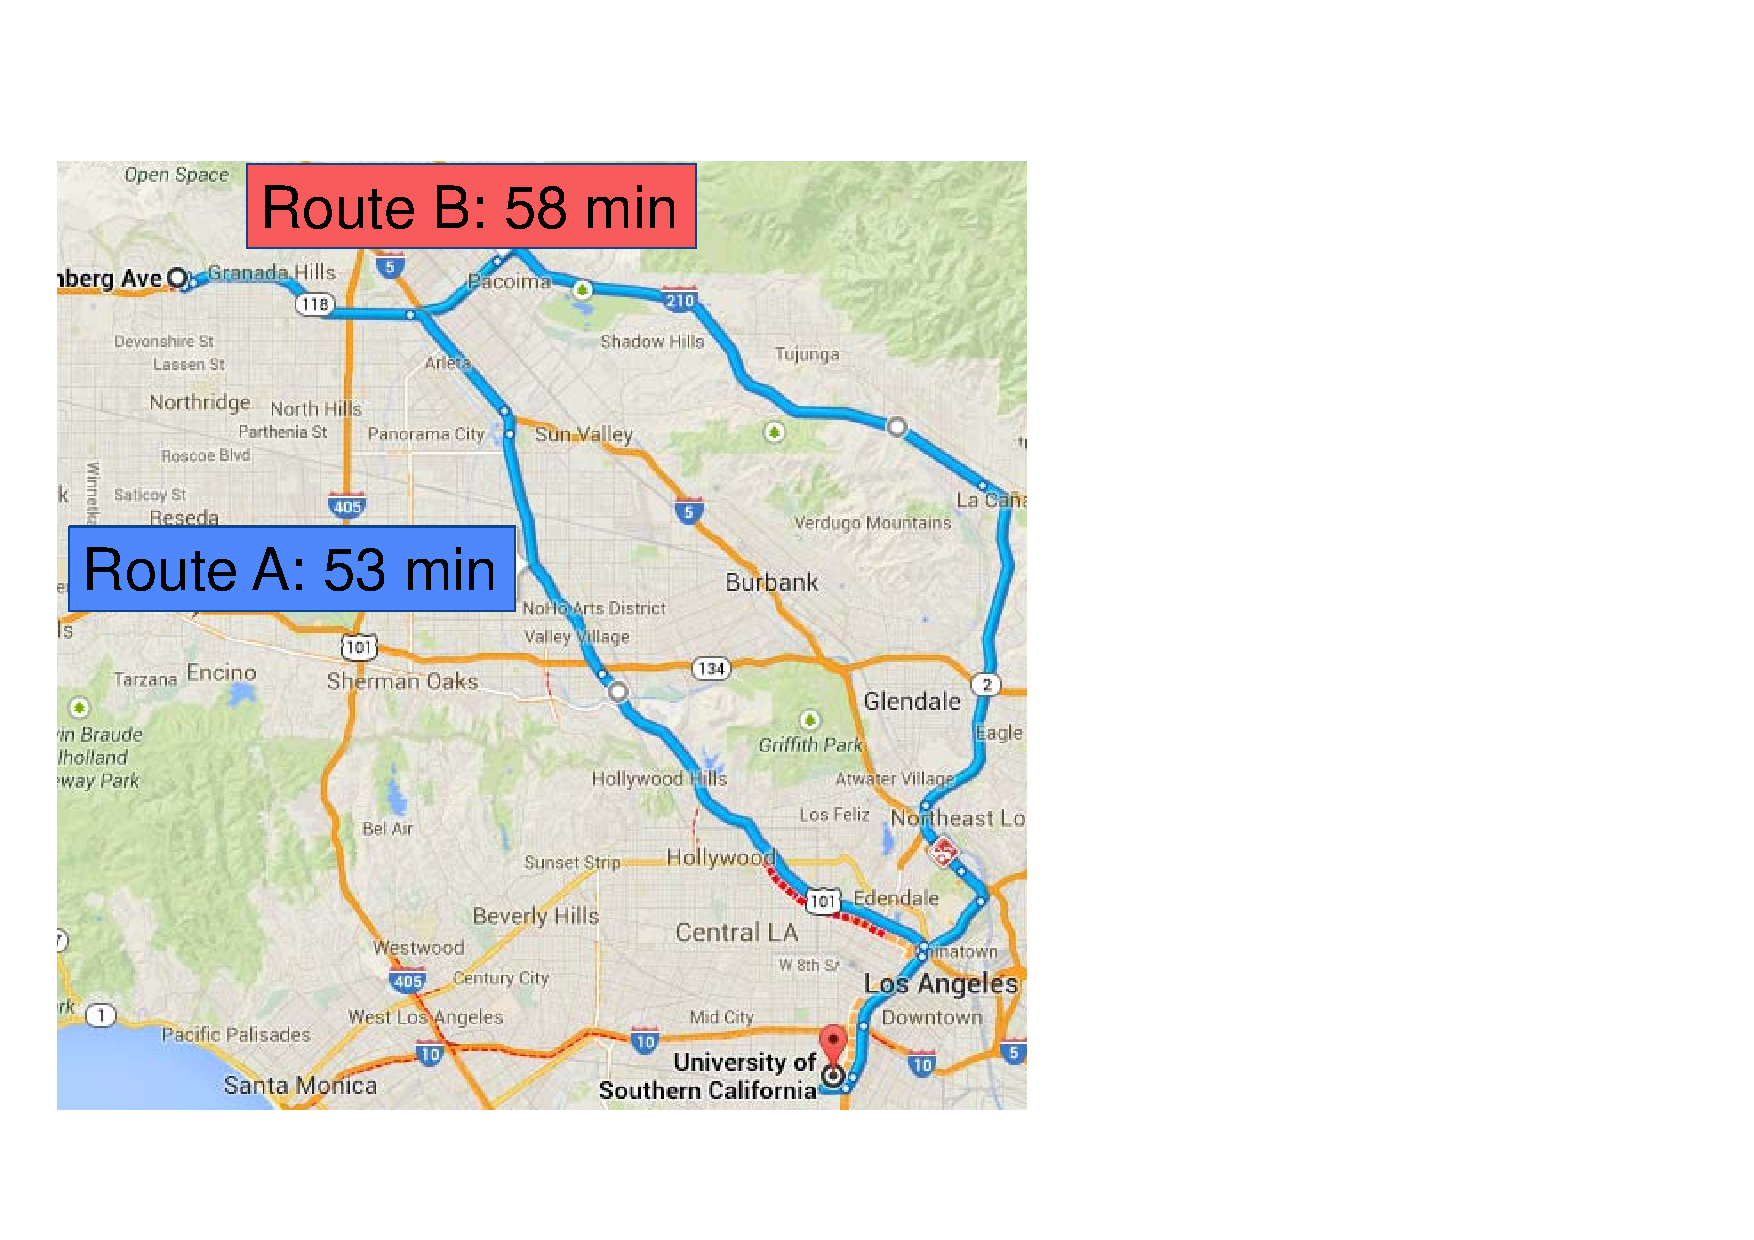
\includegraphics[scale=0.25]{motivation1.pdf}
		\end{center}
	\column{0.5\textwidth}
\end{columns}
}
\only<3->{
\begin{columns}
	\column{0.5\textwidth}
		\begin{center}
			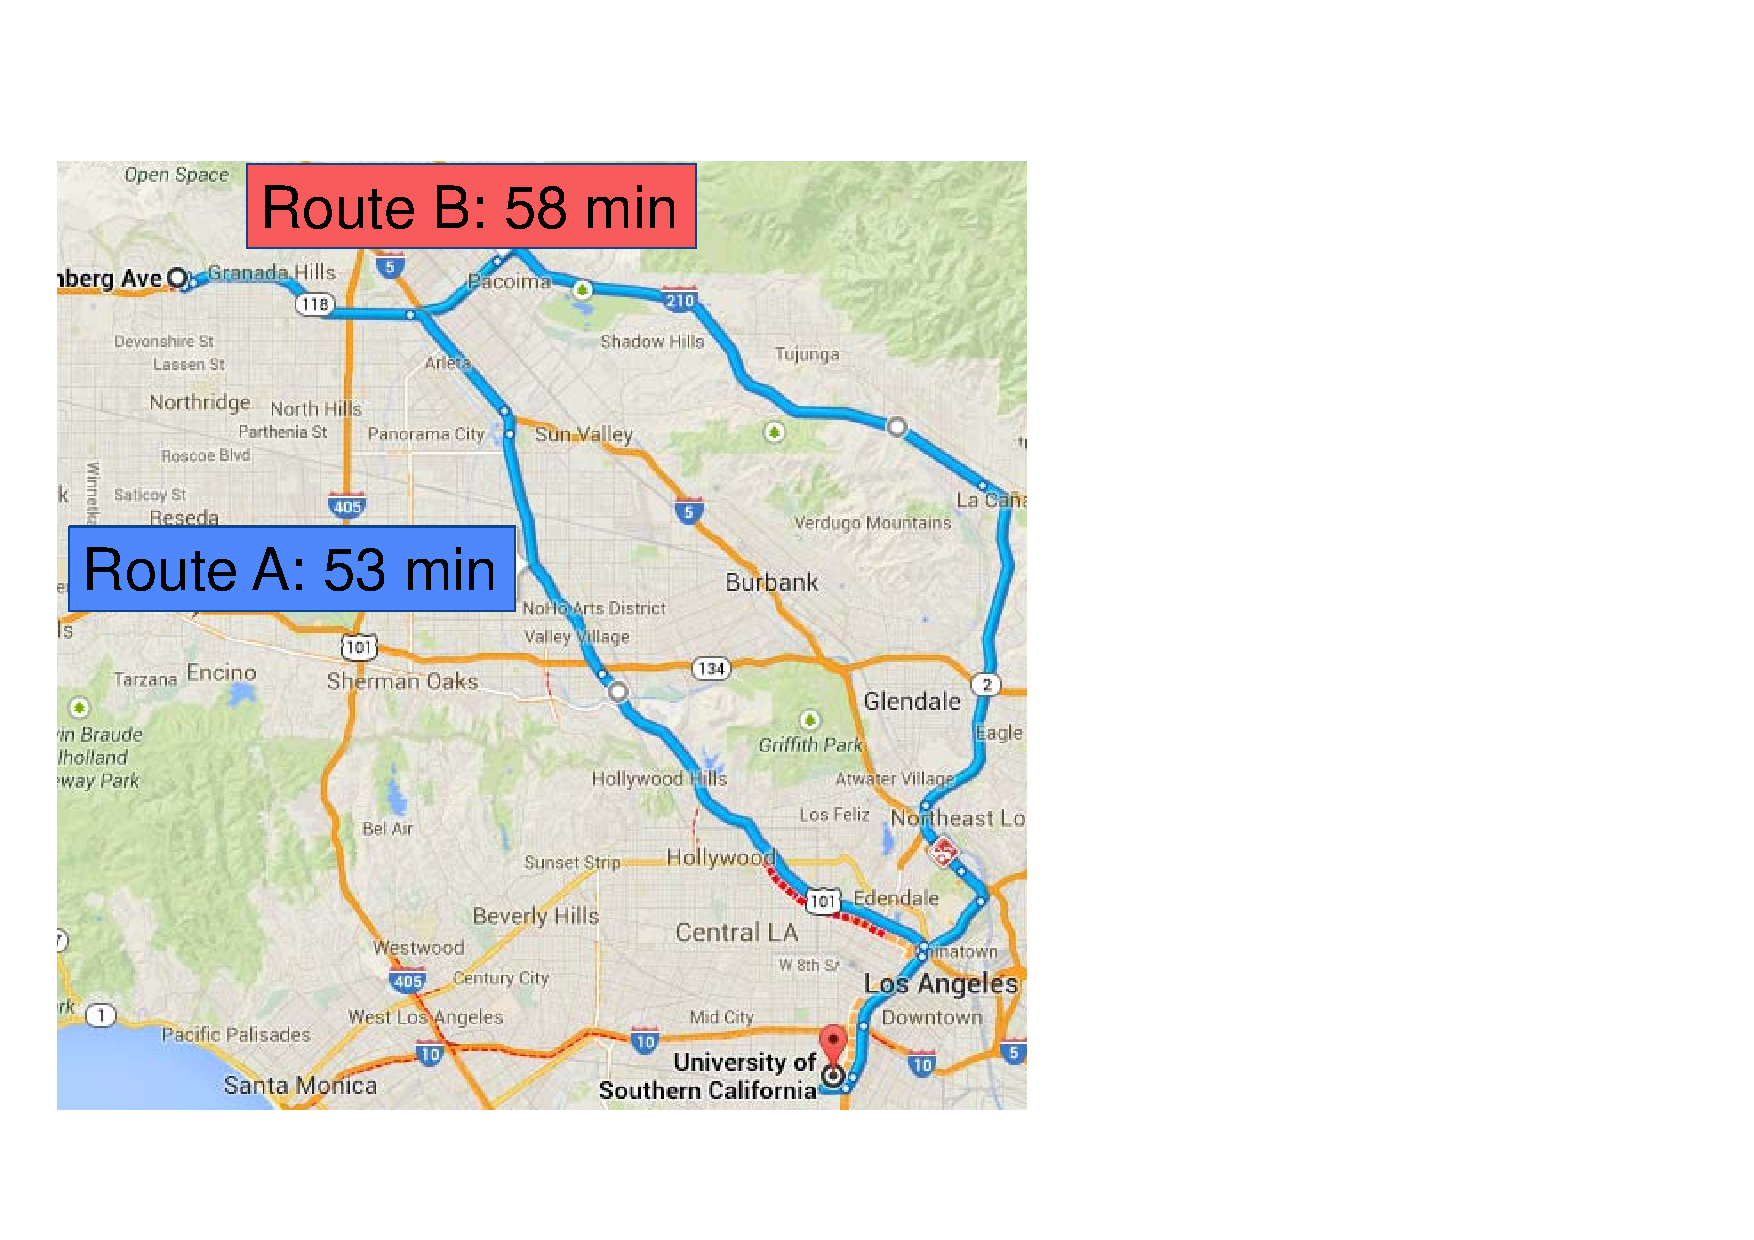
\includegraphics[scale=0.25]{motivation1.pdf}
		\end{center}
	\column{0.5\textwidth}
		\begin{center}
			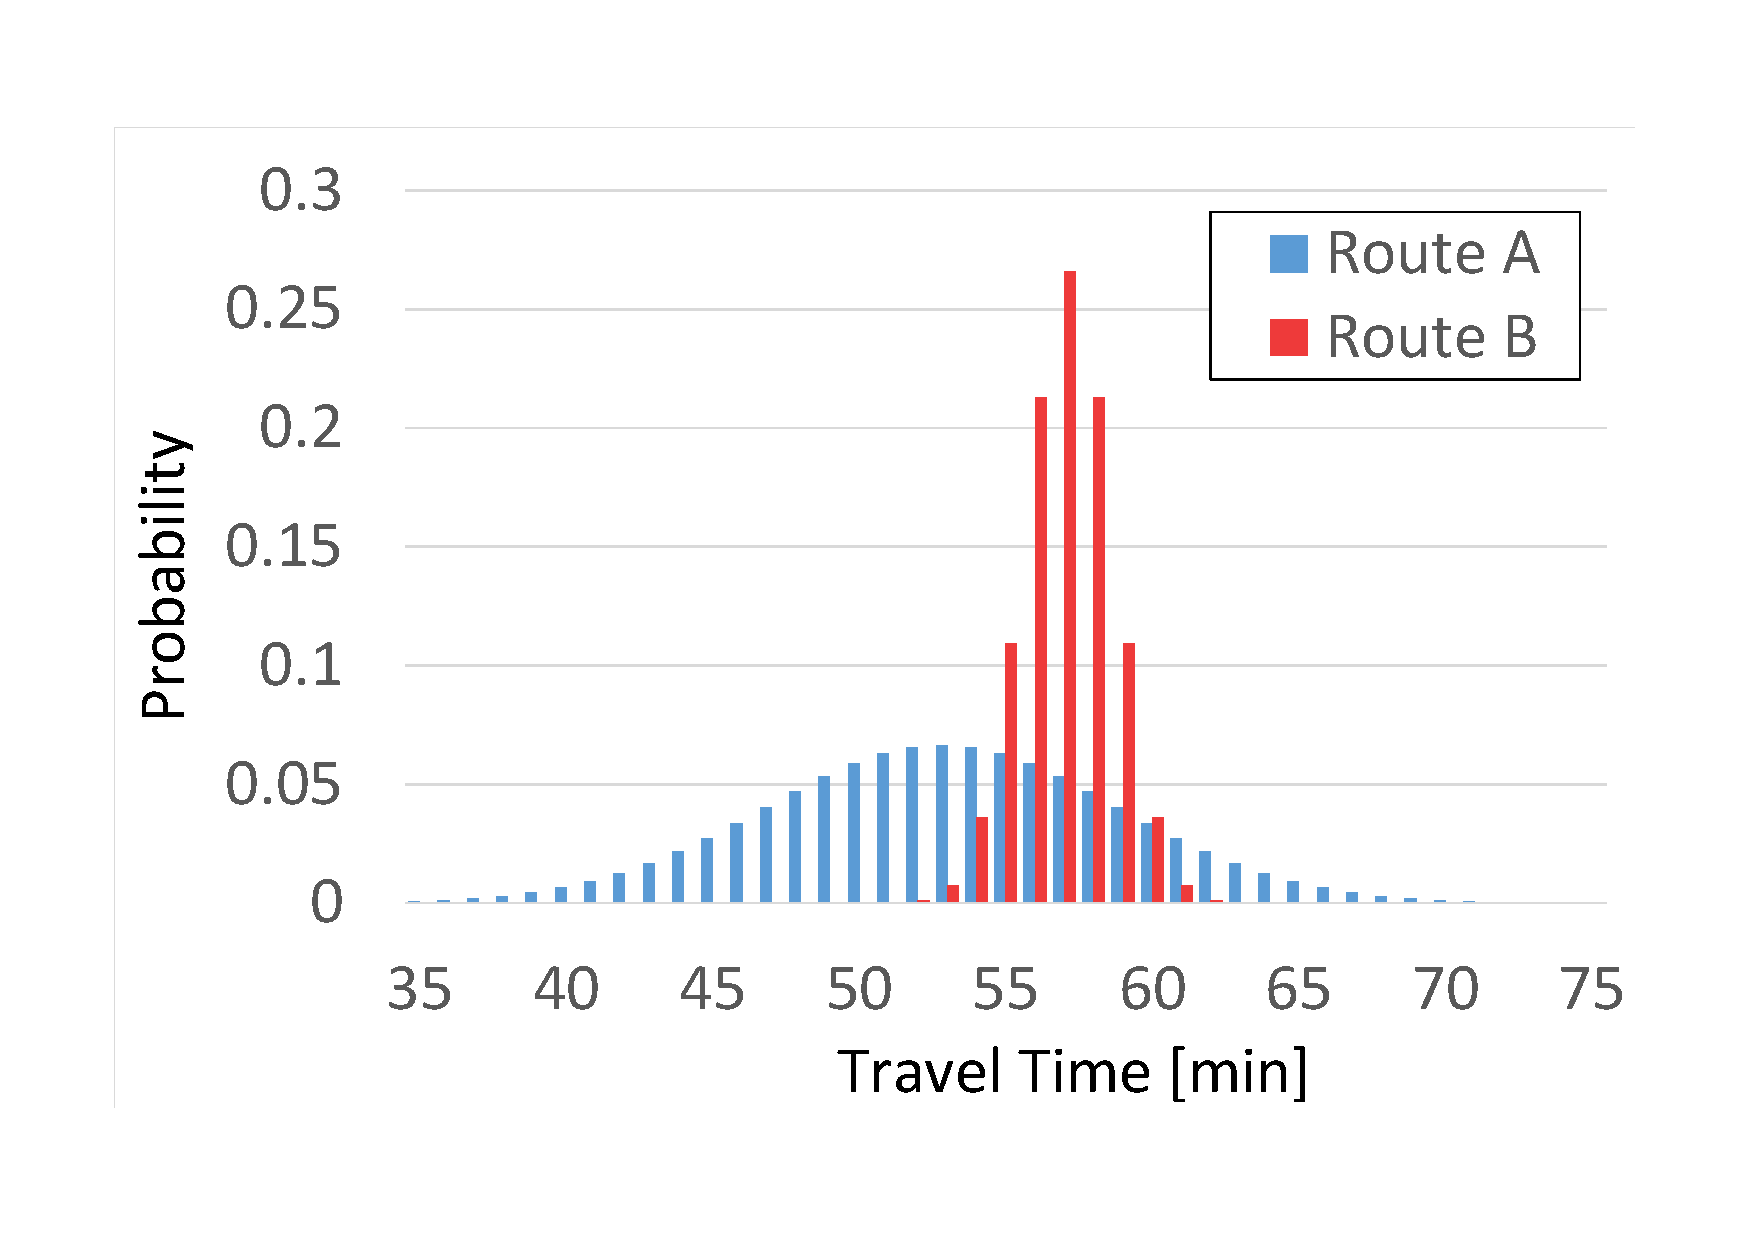
\includegraphics[scale=0.2]{motivation2.pdf}
		\end{center}
\end{columns}
}
\only<2->{
\begin{exampleblock}{}\textit{What's the probability of reaching campus in \textbf{at most} 60 minutes?}
\end{exampleblock}
}
\only<4>{
\begin{equation*}
\sum_{i \leq 60} P(i)
\end{equation*}
}
\only<5>{
\begin{itemize}
	\item \textcolor{blue}{Route A:} 89\%
	\item \textcolor{red}{Route B:} 99.2\%	
\end{itemize}
}
\end{frame}

\begin{frame}\frametitle{Probabilistic Travel Times}
\begin{columns}
\column{0.5\textwidth}
\only<2->{
How to compute the travel time \textit{PMF} for an entire route?
}
\only<3->{
\begin{itemize}
\item \tiny{H. Frank, \textit{Shortest paths in probabilistic graphs.}}
\item \tiny{E.D. Miller-Hooks et al., \textit{Least expected time paths in stochastic, time-varying transportation networks.}}
\item \tiny{Y.M. Nie et al., \textit{Shortest path problem considering on-time arrival probability.}}
\item ... 
\end{itemize}
}
\column{0.5\textwidth}
\begin{center}
	\vspace{-0.35in}
	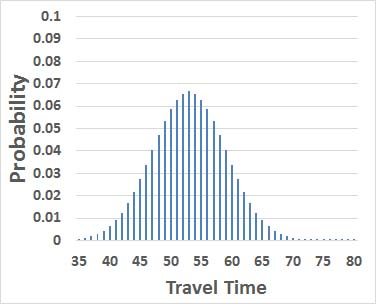
\includegraphics[scale=0.35]{Sample_PMF.jpg}
\end{center}
\end{columns}

\begin{columns}
\column{0.7\textwidth}
\only<4-5>{
\begin{center}
	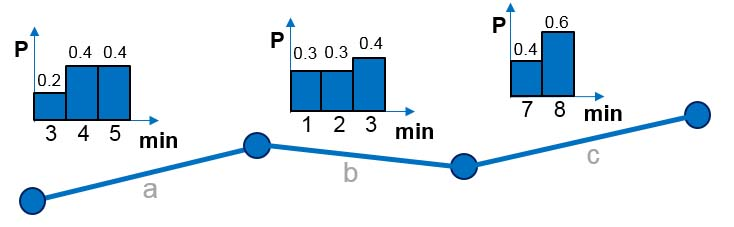
\includegraphics[scale=0.33]{route_construction1.jpg}
\end{center}
}
\only<6->{
\begin{center}
	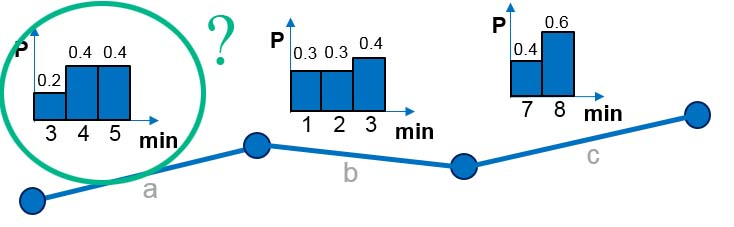
\includegraphics[scale=0.33]{route_construction2.jpg}
\end{center}
}
\column{0.3\textwidth}
\only<5->{
\begin{center}
	\vspace{0.2in}
	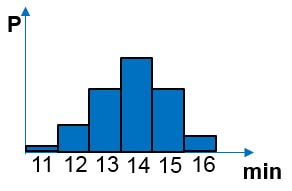
\includegraphics[scale=0.33]{sample_pmf2.jpg}
\end{center}
}
\end{columns}
\end{frame}

\section{Definitions}
\frame{\frametitle{Outline}\tableofcontents[currentsection]}

\begin{frame}\frametitle{Definitions}
\vspace{-0.2in}
\begin{block}{\textit{Probabilistic Link Travel Times \textit{(pltt)}}}
The probabilistic link travel time of link $(i,j)$, $c_{ij}^t(x)$, is the probability of taking $x$ seconds for a vehicle to traverse link $(i,j)$ starting at time $t$.
\end{block}
\only<2->{
\begin{alertblock}{Route PDF (\textbackslash PMF)}
If $p_{sd}$ is a path starting at $s$ and ending in $d$, $\pi_{sd}^t$ is the random variable representing the travel time on $p_{sd}$ when we start at time $t$. Accordingly, the route pdf, $J_{sd}^t(x)$, gives the probability of taking $x$ seconds for a vehicle to traverse $p_{sd}$ starting at time $t$
\end{alertblock}
}
\only<3>{
\begin{center}
	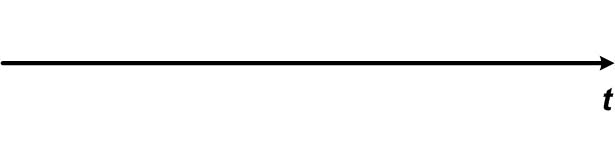
\includegraphics[scale=0.33]{times1.jpg}
\end{center}
}
\only<4>{
\begin{center}
	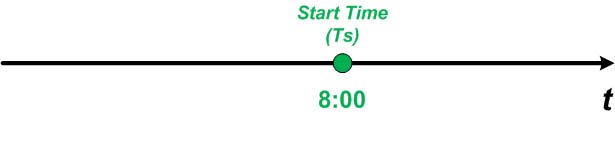
\includegraphics[scale=0.33]{times2.jpg}
\end{center}
}
\only<5>{
\begin{center}
	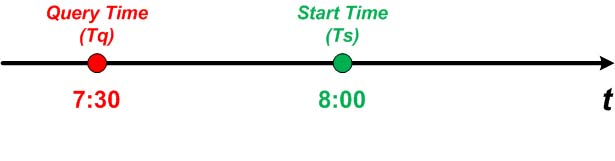
\includegraphics[scale=0.33]{times3.jpg}
\end{center}
}
\only<6>{
\begin{center}
	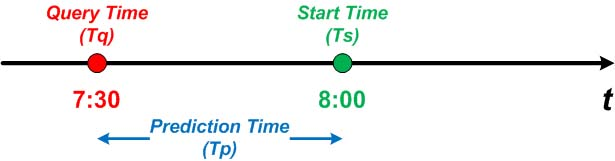
\includegraphics[scale=0.33]{times4.jpg}
\end{center}
}
\end{frame}

\section{Probabilistic Link Travel Times}
\frame{\frametitle{Outline}\tableofcontents[currentsection]}

\begin{frame}
\begin{itemize}
\item Historic Data Vs. Current Situation
\item<2-> PLTT Representation (Continuous Vs. Discrete)
\begin{itemize}
\item<3-> Continuous\\
\only<3>{
Link Travel times are normally or gamma distributed.
}
\only<4->{
Link Travel times are \textbf{normally} or gamma distributed
\begin{itemize}
\item $c_{ij}^t$ is characterized by a mean $\mu_{ij}^t$ and a standard deviation $\sigma_{ij}^t$.
\end{itemize}
}
\item<5-> Discrete\\

\only<6->{
We use b-discrete to discretize the time domain into intervals of length $\phi$:

\begin{equation*}
	T = \{ t | t = n \cdot \phi \wedge n \in \mathbb{N} \}
\end{equation*}
}

\only<7->{
Then the PMF $F_{ij}$ of link travel time $c_{ij}$ will be:
\begin{equation*}
	F_{ij}(b) = \begin{cases}\int_b^{b+\phi}f_{ij}(w)dw \qquad b =
	0,\phi,\ldots, (L-1)\phi\\
	\int_b^{\infty}f_{ij}(w)dw \qquad b =
	L \phi\\
	0 \qquad otherwise
	\end{cases} 
\end{equation*}
}
\end{itemize}
\end{itemize}
\end{frame}

\begin{frame}\frametitle{Historic Data}
\begin{equation*}
H = \{h | h < t_q\}
\end{equation*}

\begin{itemize}
\item<2-> Which historic data should we use?
\end{itemize}
\vspace{0.25in}
\only<3->{
\begin{equation*}
H^{t_s} \subset H
\end{equation*}
}
\only<4->{
\begin{exampleblock}{}
\begin{center}
At a specific \textbf{time of day}, the traffic follows similar patterns during \textbf{weekdays}.\\
\end{center}
\tiny{* B. Pan et. al., \textit{Utilizing real-world transportation data for accurate traffic prediction}.}
\end{exampleblock}
}
\end{frame}

\begin{frame}\frametitle{Historic Data \small{(cont'd)}}
\begin{itemize}
\item Continuous
\begin{gather*}
	\mu_{ij}^{t_s} = \frac{1}{|H^{t_s}|}\sum_{h\in H^{t_s}} c_{i,j}^h\\ 
	(\sigma_{ij}^{t_s})^2 = \frac{1}{|H^{t_s}|}\sum_{h\in H^{t_s}} (c_{ij}^h-\mu_{ij}^{t_s})^2\\
	\rho_{ij-kl} = \frac{\sum_{h\in H^{t_s}} (c_{ij}^h - \mu_{ij}) (c_{kl}^h -
	\mu_{kl})}{(|H^{t_s}|-1) \sigma_{ij} \sigma_{kl}}
\end{gather*}
\item<2-> Discrete
\only<2->{
\begin{gather*}
  F_{ij}^{t_s}(b) = \frac{1}{|H^{t_s}|}\sum_{h\in H^{t_s}} I(\lceil c_{ij}^h \rceil^\phi= b)
\end{gather*}
}
\end{itemize}
\end{frame}

\begin{frame}\frametitle{Historic Data \small{(cont'd)}}
\vspace{-0.45in}
\begin{columns}
\column{0.5\textwidth}
	\begin{figure}
		\centering
		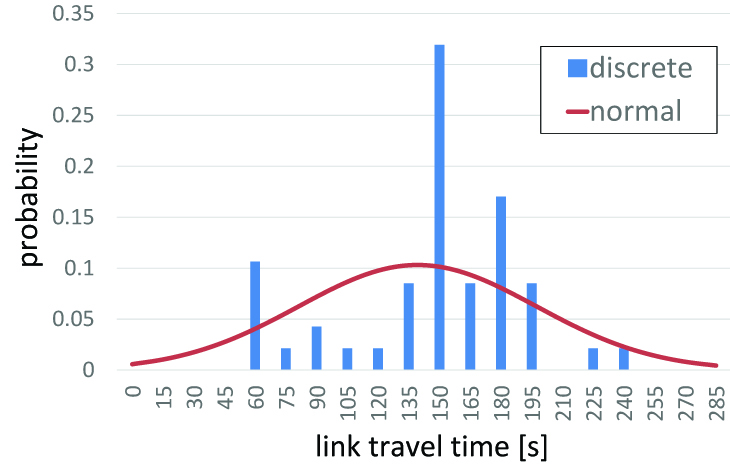
\includegraphics[scale=0.2]{ltt_0900.jpg}
		\vspace{-0.05in}
		\\ 09:00AM
	\end{figure}
\column{0.5\textwidth}
	\begin{figure}
		\centering
		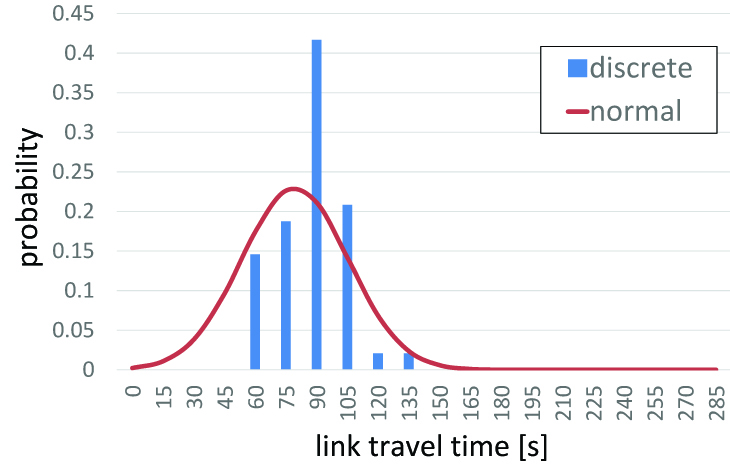
\includegraphics[scale=0.2]{ltt_1200.jpg}
		\vspace{-0.05in}
		\\ 12:00PM
	\end{figure}
\end{columns}
\begin{center}
	\begin{figure}
		\centering
		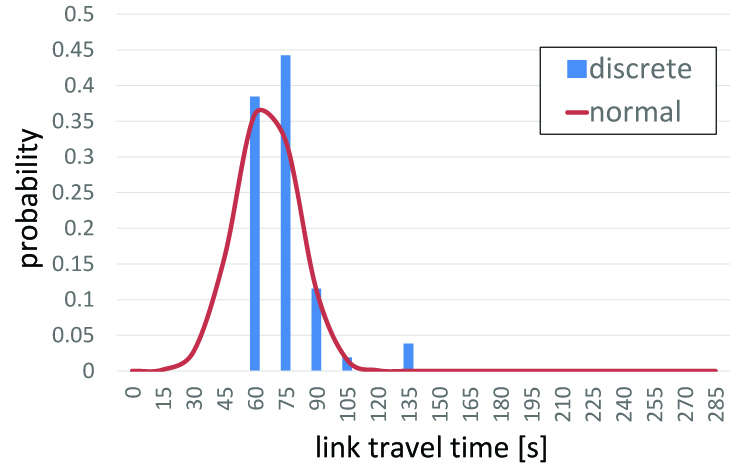
\includegraphics[scale=0.2]{ltt_1800.jpg}	
		\vspace{-0.05in}
		\\ 06:00PM
	\end{figure}
\end{center}

\end{frame}

\begin{frame}\frametitle{Similar Historic}
\only<1>{
\begin{center}
	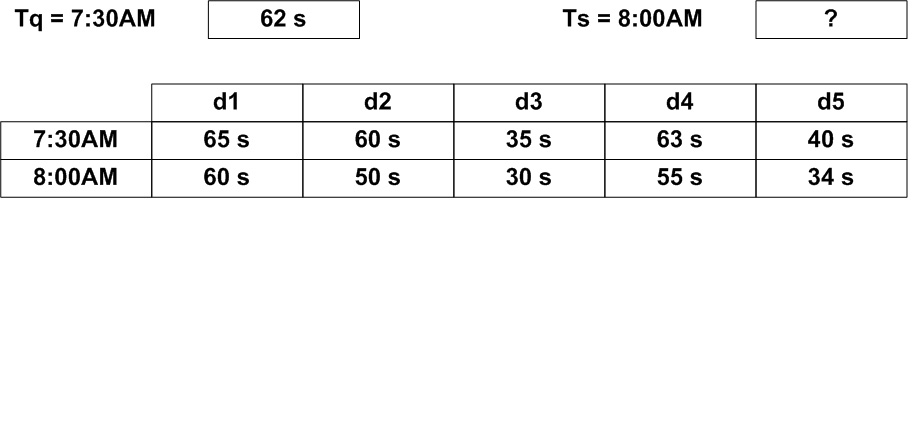
\includegraphics[scale=0.35]{similar_historic1.jpg}
\end{center}
}
\only<2>{
\begin{center}
	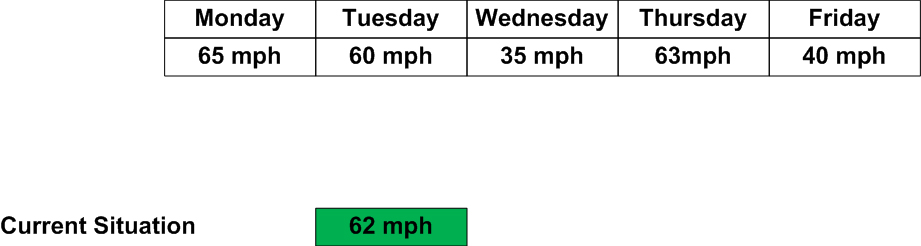
\includegraphics[scale=0.35]{similar_historic2.jpg}
\end{center}
}
\only<3>{
\begin{center}
	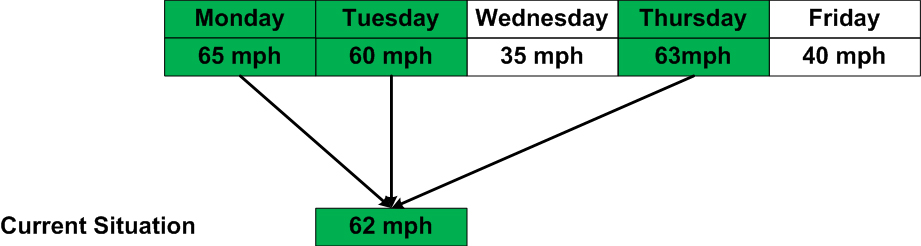
\includegraphics[scale=0.35]{similar_historic3.jpg}
\end{center}
}
\only<4->{
\begin{center}
	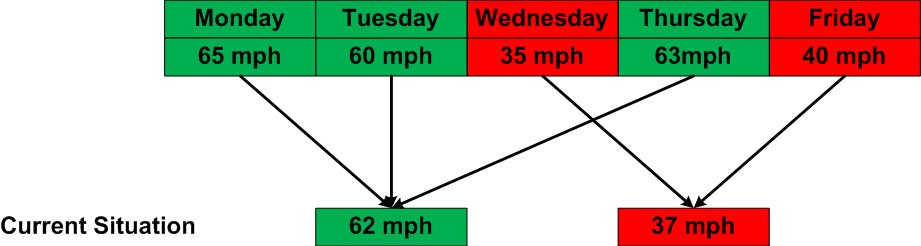
\includegraphics[scale=0.35]{similar_historic4.jpg}
\end{center}
}
\only<5->{
\vspace{0.75in}
\begin{equation*}
H_{i,j}^{t_s} = \{h|h \in H^{t_s} \wedge \left| \frac{c_{i,j}^{t_q} - c_{i,j}^{h-t_p}}{c_{i,j}^{t_q}} \right| \leq \lambda \}  
\end{equation*}
}
\end{frame}

\begin{frame}\frametitle{Linear Interpolation}
\only<1>{
\begin{center}
	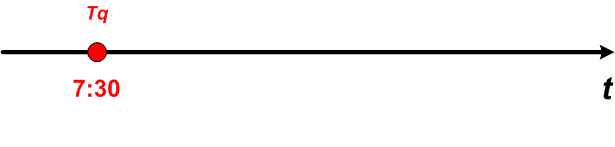
\includegraphics[scale=0.45]{time_horizon1.jpg}
\end{center}
}
\only<2>{
\begin{center}
	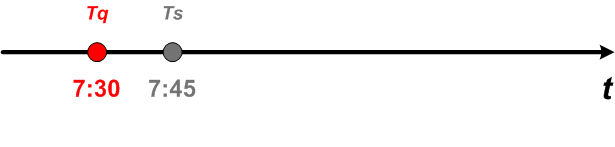
\includegraphics[scale=0.45]{time_horizon2.jpg}
\end{center}
}
\only<3>{
\begin{center}
	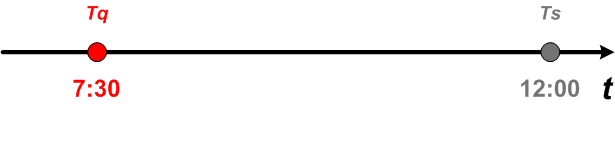
\includegraphics[scale=0.45]{time_horizon3.jpg}
\end{center}
}
\only<4->{
\begin{center}
	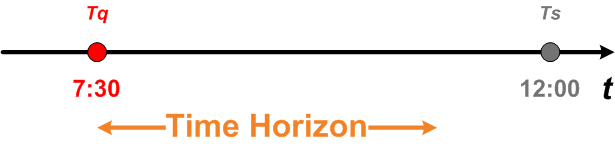
\includegraphics[scale=0.45]{time_horizon4.jpg}
\end{center}
}
\begin{itemize}
\item<5-> Time Horizon $\rightarrow \tau$
\item<6-> $\theta = min \{\frac{t_p}{\tau}, 1 \}$
\end{itemize}
\end{frame}

\begin{frame}\frametitle{Linear Interpolation \small{(cont'd)}}
\begin{itemize}
\item<1-> Continuous
\only<1->{
\begin{gather*}
	\mu_{ij}^{t_s} = \left(\theta\cdot\frac{1}{|H^{t_s}|}\sum_{h\in H^{t_s}} c_{i,j}^h \right)
	+ \left(1-\theta\right)\cdot c_{i,j}^{t_q}\\
	(\sigma_{ij}^{t_s})^2 = \theta^2 \cdot \frac{1}{|H^{t_s}|}\sum_{h\in H^{t_s}}
	(c_{ij}^h-\mu_{ij}^{t_s})^2
\end{gather*}
}
\item<2-> Discrete
\only<2->{
\begin{gather*}
F_{ij}^{t_s}(b) = \frac{1}{|H^{t_s}|}\sum_{h\in H^{t_s}} I(\lceil\theta \cdot 
c_{ij}^h + (1-\theta)\cdot c_{i,j}^{t_q}\rceil^\phi = b)
\end{gather*}
}
\end{itemize}

\end{frame}

\begin{frame}\frametitle{Linear Interpolation \small{(cont'd)}}
\begin{figure}
    \centering
    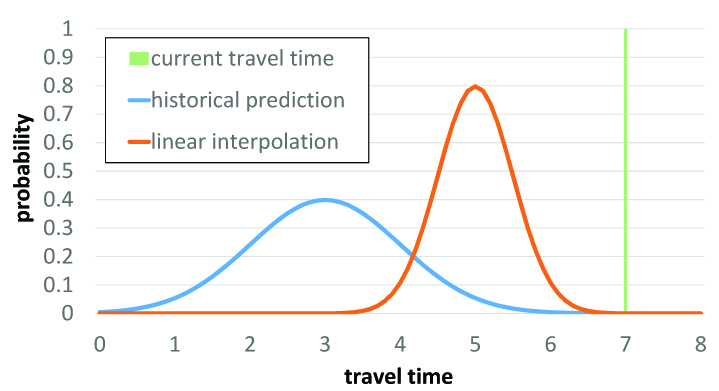
\includegraphics[width=0.80\columnwidth]{tt_interpolation.jpg}\\
    Linear Interpolation example with $\theta = 0.5$
\end{figure}
\end{frame}

\section{Route Reliability Computation}
\frame{\frametitle{Outline}\tableofcontents[currentsection]}

\begin{frame}\frametitle{Route PDF (\textbackslash PMF) Classification}
\begin{itemize}
\item Continuous Vs. Discrete Link Models
\item<2-> Time-Dependent Vs. Static
\item<3-> Correlated Vs. Independent
\end{itemize}
\only<4>{
\begin{table}
\centering
\begin{tabular}{| l || c | c | c | c|}
\hline
Method & Link model & Time-dependency & Correlation \\
\hline    \hline
ConStaInd & continuous  & no & no\\ \hline
DisStaInd & discrete & no & no\\ \hline
ConTimInd & continuous & yes & no\\ \hline
DisTimInd & discrete & yes & no\\ \hline
ConStaCor & continuous & no & yes\\ \hline
DisStaCor & discrete & no & yes\\ \hline
ConTimCor & continuous & yes & yes\\ \hline
DisTimCor & discrete & yes & yes\\ \hline
\end{tabular}
\end{table}
}
\only<5>{
\begin{table}
\centering
\begin{tabular}{| l || c | c | c | c|}
\hline
Method & Link model & Time-dependency & Correlation \\
\hline    \hline
\rowcolor{blue!25}
ConStaInd & continuous  & no & no\\ \hline
\rowcolor{blue!25}
DisStaInd & discrete & no & no\\ \hline
ConTimInd & continuous & yes & no\\ \hline
\rowcolor{blue!25}
DisTimInd & discrete & yes & no\\ \hline
\rowcolor{blue!25}
ConStaCor & continuous & no & yes\\ \hline
DisStaCor & discrete & no & yes\\ \hline
ConTimCor & continuous & yes & yes\\ \hline
DisTimCor & discrete & yes & yes\\ \hline
\end{tabular}
\end{table}
}
\end{frame}

\begin{frame}\frametitle{Route PDF (\textbackslash PMF) Computation Methods}
\begin{itemize}
\item \textbf{ConStaInd}
\only<1>{
\begin{gather*}
	\mu_{p} = \sum_{(i,j)\in p} \mu_{ij} \text{ and } \sigma_{p}^2 =
	\sum_{(i,j)\in p} \sigma_{ij}^2 
\end{gather*}
}
\item<2-> \textbf{DisStaInd}
\only<2>{
\begin{gather*}
	J_{sj}(b) = \sum_{h=0}^b J_{si}(b-h) F_{ij}(h)  , \forall b = 0, \phi,\ldots, L
	\phi
\end{gather*}
}
\item<3-> \textbf{DisTimInd}
\only<3>{
\begin{gather*}
	J_{sj}(b) = \sum_{h=0}^b J_{si}(b-h) F_{ij}^{b-h}(h)  , \forall b = 0,
	\phi,\ldots, L
	\phi
\end{gather*}
}
\item<4-> \textbf{ConStaCor}
\only<4>{
\begin{gather*}
	\mu_{p} = \sum_{(i,j)\in p} \mu_{ij}, \\
	\sigma_{p}^2 = \sum_{(i,j)\in p} \sigma_{ij}^2 +\sum_{(i,j)\neq(k,l)\in p}
	\rho_{ij-kl}
	\sigma_{ij} \sigma_{kl}
\end{gather*}
}
\end{itemize}
\end{frame}

\section{Evaluating Probabilistic Predictions}
\frame{\frametitle{Outline}\tableofcontents[currentsection]}

\section{Experiments}
\frame{\frametitle{Outline}\tableofcontents[currentsection]}

\begin{frame}\frametitle{Data Set}

\begin{itemize}
\item<2-> 50 links of $\sim 1$ mile.
\item<3-> 10 routes of $\sim 40$ mile.
\end{itemize}
\end{frame}

\begin{frame}\frametitle{Methodology}
\begin{itemize}
\item Start Times: 8:00AM, 9:00AM, 4:00PM, 5:00PM, 6:00PM during weekdays in 2013\\
\only<2->{$\rightarrow 5$ days $\times \ 52$ weeks $ = 260$ sample for each start time}.
\item<3-> We use k-fold cross validation (k = 5).
\end{itemize}

\end{frame}

\begin{frame}\frametitle{Historic}
\vspace{0.5in}
\begin{columns}
	\column{0.5\textwidth}
		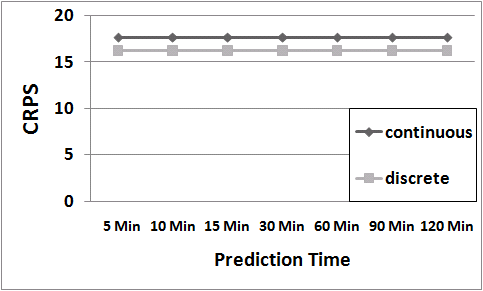
\includegraphics[scale=0.3]{Links_Historic.png}
	\column{0.5\textwidth}
		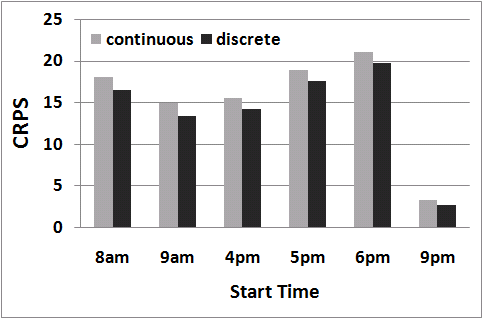
\includegraphics[scale=0.3]{Links_Historic_TOD.png}
\end{columns}
\end{frame}

\begin{frame}\frametitle{Similar Historic}
\begin{center}
	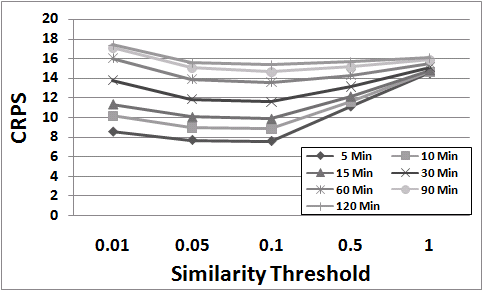
\includegraphics[scale=0.5]{Links_Filtered.png}
\end{center}
\end{frame}

\begin{frame}\frametitle{Linear Interpolation}
\vspace{0.5in}
\begin{columns}
	\column{0.5\textwidth}
		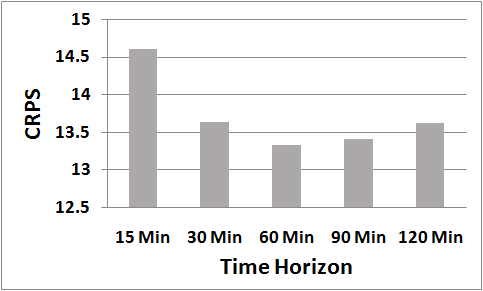
\includegraphics[scale=0.3]{Links_Interpolated_TimeHorizon.png}
	\column{0.5\textwidth}
		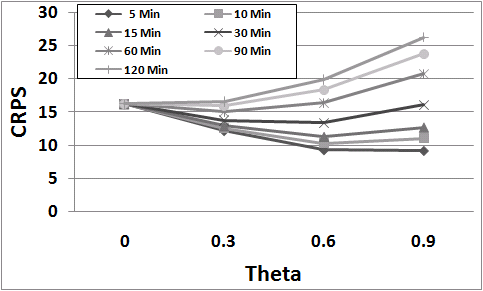
\includegraphics[scale=0.3]{Links_Interpolated_Theta.png}
\end{columns}
\end{frame}

\begin{frame}\frametitle{Best Parameters}
\begin{center}
	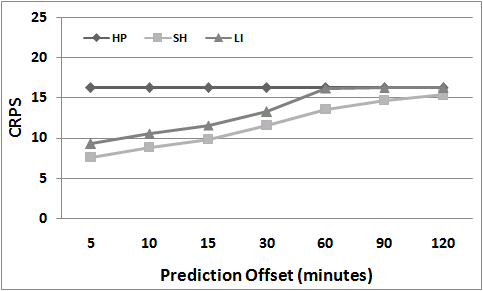
\includegraphics[scale=0.5]{Links_Best.png}
\end{center}
\end{frame}

\begin{frame}\frametitle{Routes}
\vspace{-0.35in}
\begin{columns}
	\column{0.5\textwidth}
		\begin{center}
			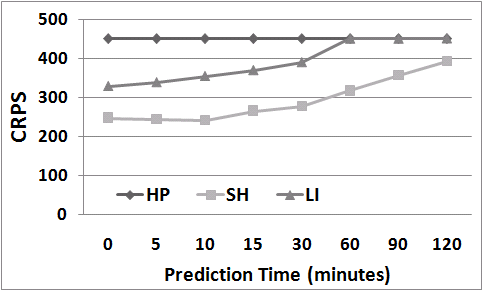
\includegraphics[scale=0.3]{Approaches_ConStaInd.png}\\
			ConStaInd
		\end{center}
	\column{0.5\textwidth}
		\begin{center}
			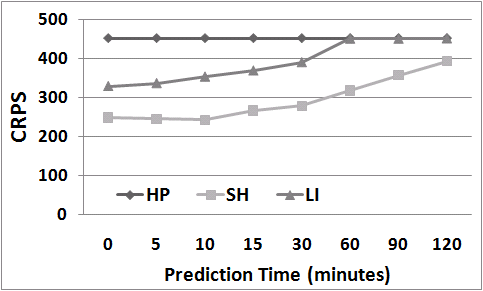
\includegraphics[scale=0.3]{Approaches_DisStaInd.png}\\
			DisStaInd
		\end{center}
\end{columns}
\begin{columns}
	\column{0.5\textwidth}
		\begin{center}
			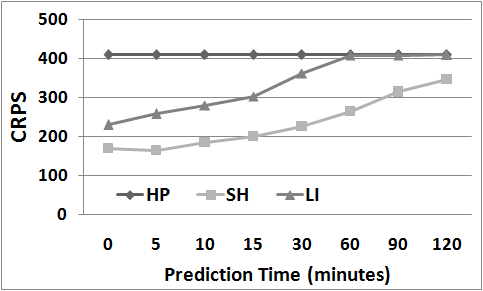
\includegraphics[scale=0.3]{Approaches_DisTimInd.png}\\
			DisTimInd
		\end{center}
	\column{0.5\textwidth}
		\begin{center}
			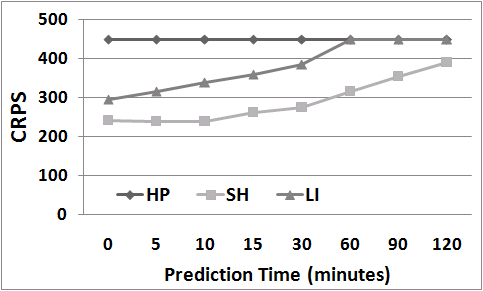
\includegraphics[scale=0.3]{Approaches_ConStaCor.png}\\
			ConStaCor
		\end{center}
\end{columns}
\end{frame}

\begin{frame}\frametitle{Routes \small{(cont'd)}}
\vspace{0.5in}
\begin{center}
	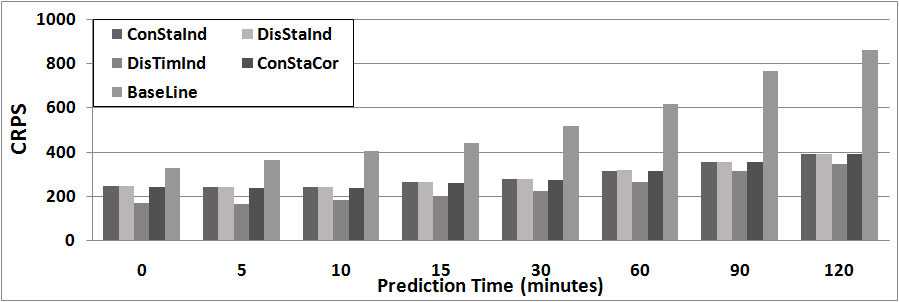
\includegraphics[scale=0.3]{Approaches_All.png}
\end{center}
\end{frame}


\section{Q \& A}
\frame{\frametitle{Outline}\tableofcontents[currentsection]}



\end{document}